
%(BEGIN_QUESTION)
% Copyright 2011, Tony R. Kuphaldt, released under the Creative Commons Attribution License (v 1.0)
% This means you may do almost anything with this work of mine, so long as you give me proper credit

Determine how either of the potentiometers may be connected to the temperature transmitter in order to simulate a 4-wire RTD:

$$\includegraphics[width=15.5cm]{i03567x01.eps}$$

\vskip 20pt \vbox{\hrule \hbox{\strut \vrule{} {\bf Suggestions for Socratic discussion} \vrule} \hrule}

\begin{itemize}
\item{} Students very commonly mis-interpret the symbols drawn next to the input terminals of an RTD transmitter, especially the terminals which must be made common to each other at the sensor.  One of the most popular misconceptions  is to think that those terminals shown common to each other by the symbol are already joined together {\it inside the transmitter}.  Explain why this interpretation cannot be true, based on how you know 3-wire and 4-wire RTD circuits are designed to work.
\item{} A problem-solving technique useful for making proper connections in pictorial circuit diagrams is to first identify the directions of all DC currents entering and exiting component terminals, as well as the respective voltage polarity marks (+,$-$) for those terminals, based on your knowledge of each component acting either as an electrical {\it source} or an electrical {\it load}.  Discuss and compare how these arrows and polarity marks simplify the task of properly connecting wires between components. 
\item{} Perhaps the most difficult part of this problem is deciding how to connect the potentiometer to the transmitter.  One way to help you solve this problem is to apply the technique of {\it simplifying} the problem so that it is easier to solve, then use that solution as a starting point for the final solution of the given (complex) problem.  Show how you would first simplify the given problem here, and what that simple(r) solution would look like.
\end{itemize}

\underbar{file i03567}
%(END_QUESTION)





%(BEGIN_ANSWER)


%(END_ANSWER)





%(BEGIN_NOTES)

These are some possible solutions, but by no means the only solutions:

$$\includegraphics[width=15.5cm]{i03567x02.eps}$$

$$\includegraphics[width=15.5cm]{i03567x03.eps}$$

%INDEX% Measurement, temperature: RTD resistance calibration

%(END_NOTES)


